\section{\textbf{Own approach }}\label{sec:main}
 
 
This part will identify TSN requirements over 5G testbed and the automatic setup of selected open-source 5G testbed.
 \subsection{The integration of 5G with TSN configuration approach}
 
The Thesis will deal with the use cases of integration 5G-TSN  in the Manufacturing Domains, where 5G technology does not has any action on  E2E protocols. I.e., This refers to the transparent methods of 5G-TSN integration\cite{Neumann2018}. On the contrary, the study will not discuss the non-transparent methods of 5G-TSN integration presented by Tunneling, gateways, and proxies. By reason of not being able to meet requirements of the combining of 5G and TSN.

 
Other related concepts are P802.1Qcc, and Stream Reservation Protocol (SRP) Enhancements and Performance Improvements \cite{TSN2019_study}. 802.1Qcc enables the coexistence between centralized configuration management and decentralized configuration, configurable SR (stream reservation) classes and streams, benefits heterogeneous configurations for legacy Audio Video Bridging (AVB) equipment \cite{kreifeldt2009avb}, support for Layer 3 streaming, fully centralized configuration, deterministic stream reservation convergence, and fully distributed configuration of the Stream Reservation Protocol (SRP)\cite{TSN2019_study}. TSN Configuration fully distributed model showed in figure \textbf{\ref{fig:TSN_Configuration_fullydistributed[802.1Qcc]}}.
\begin{itemize}
    \item Fully centralized configuration of IEEE 802.1Qcc: Regarding IEEE 802.1 sense, the system is classified into two characters of equipment: bridges and end stations (Talker or Listener) \cite{TSN2019_study}.
    The talker end station is the source or a machine that generates data, e.g.,  (sensors). The listener end station is the destination or a machine that receives and uses data, e.g., controller or monitoring device \cite{Eri_Gar_Theo_Oper_TSN2017study}. Stream: a unidirectional movement of data from a Talker to one or more further Listeners. As depicted in 
    figure \textbf{\ref{fig:802.1Qcc_Fully_Centralized_Configuration_Model}},  the technology consists of the following elements: Centralized User Configuration (CUC), Centralized Network Controller (CNC), and Bridges. The Bridge is a design , see figure \textbf{\ref{fig:Bridge_Architecture}}, that includes Media Access Control (MAC) Bridge or Virtual Local Area Network (VLAN) Bridge element functionality \cite{Mannweiler2020}. Time-synchronization is at a high level in this topology. I.e., The topology has a collection of time-aware bridges. On the other hand, end stations and these bridges are synchronized to a master clock in the system. Besides, the complete network is sensible of the global time—however, The interaction between the previously mentioned elements detailed in figure \textbf{\ref{fig:CUC-CNC_Interactions_for_Industrial_TSN_Domain_Configuration}}. In addition, (CNC) deals with network devices (bridges), while (CUC) deals with user devices (end stations). The CNC and CUC present the control plane (CP) rather than distributed protocols; i.e., the fully centralized configuration model attends a software-defined networking (SDN) approach. In opposition, distributed control protocols are utilized in the fully distributed model, where there is no CNC or CUC \cite{Ericsson2019}.


    \begin{figure}
    \centering
    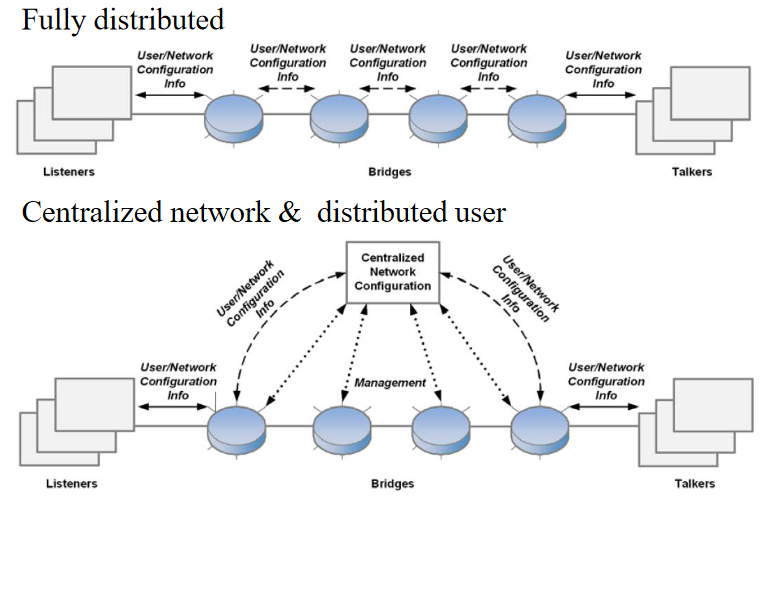
\includegraphics[scale=0.65]{images/TSN Configuration fully distributed [802.1Qcc].png} 
    \caption{TSN Configuration fully distributed [802.1Qcc] \cite{TSN2019_study}.}
    \label{fig:TSN_Configuration_fullydistributed[802.1Qcc]}
     \end{figure}
    
    
    \begin{figure}
    \centering
    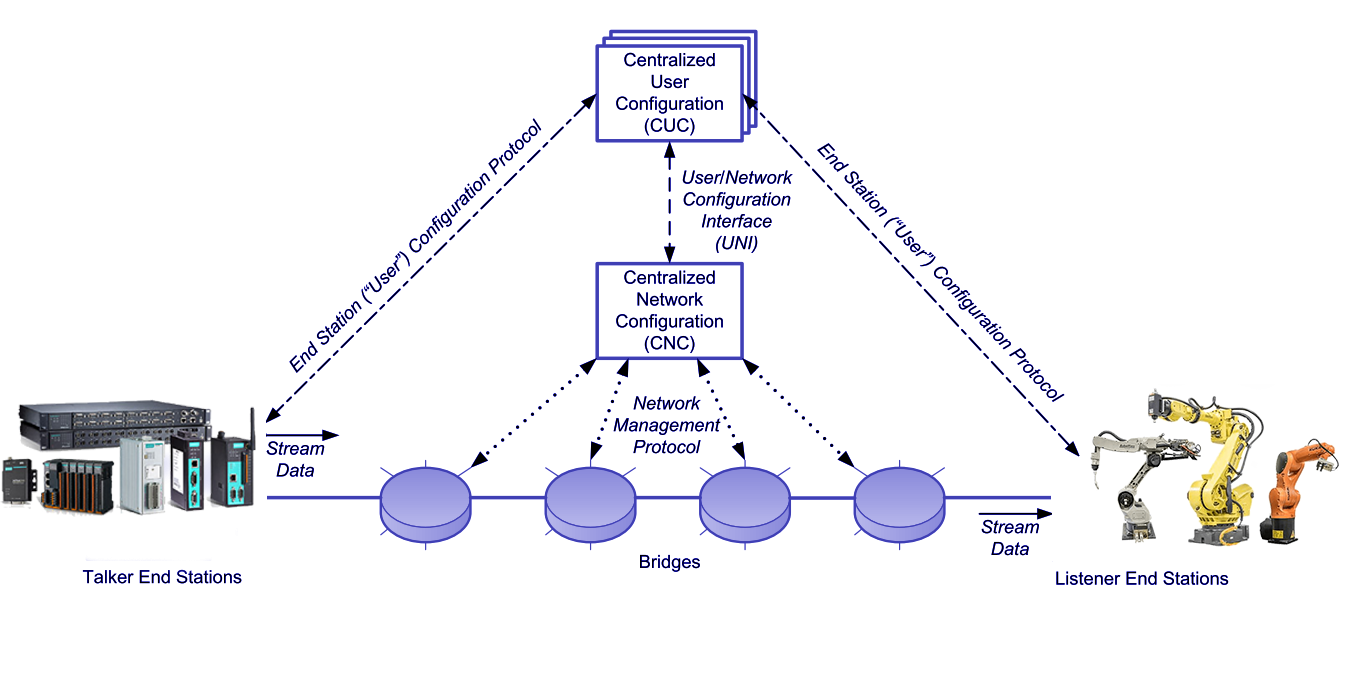
\includegraphics[scale=0.22]{images/802.1Qcc Fully Centralized Configuration Model.png} 
    \caption{802.1Qcc Fully Centralized Configuration Model \cite{Ginthor2019}}
    \label{fig:802.1Qcc_Fully_Centralized_Configuration_Model}
    \end{figure}


\begin{figure}
\centering
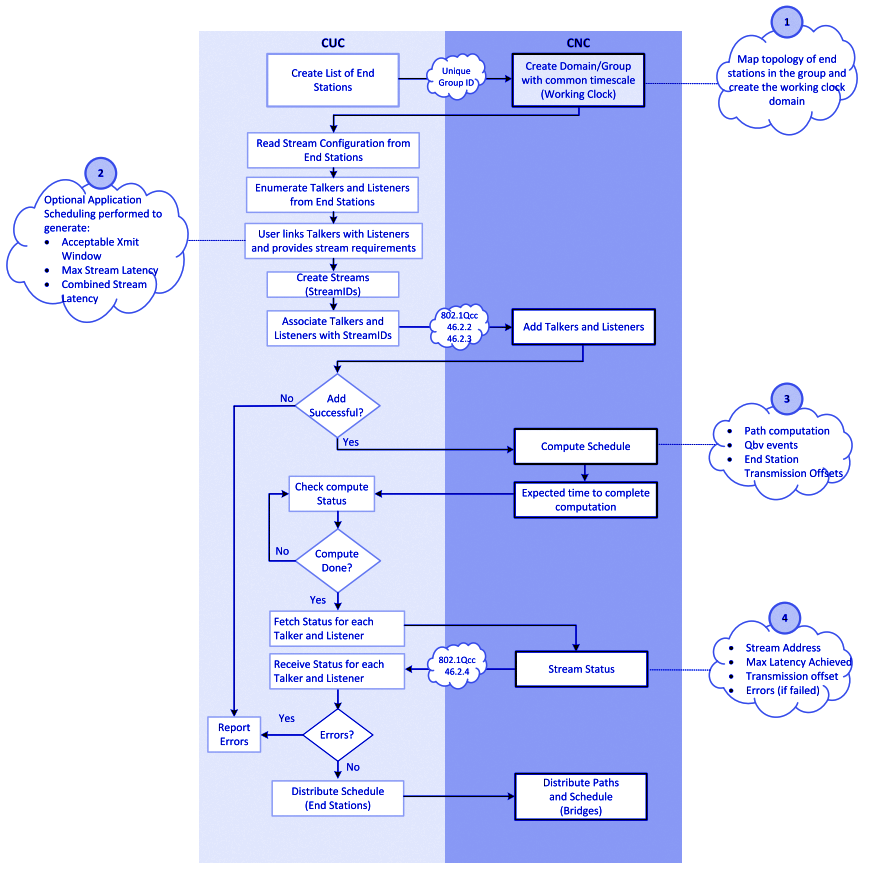
\includegraphics[scale=0.38]{images/CUC-CNC Interactions for Industrial TSN Domain Configuration.png} 
\caption{CUC-CNC Interactions for Industrial TSN Domain Configuration \cite{Eri_Gar_Theo_Oper_TSN2017study}.}
\label{fig:CUC-CNC_Interactions_for_Industrial_TSN_Domain_Configuration}
 \end{figure}


 
     \item 3GPP 5GS mobile network within TSN Transparent integration:
     In order to focus on the thesis goal, we perform a zoom in on a TSN bridge of the 802.1Qcc Fully Centralized Configuration Model, that illustrates in figure \textbf{\ref{fig:OS-5GC-Main}} considering TSN features that shown in figure
     \textbf{\ref{fig:TSN_toolbox}}. 
       Regarding 3GPP Release 16, two operative items are provided; TSN Translator (TT) and an adaptation interface (AIF). Both items represent the concept of the integration of 5G into TSN in industrial automation. I.e., TT and AIF encapsulate the 5G network as a virtual bridge in the TSN network. These two objects modify the TSN performances into identical movements in the 5G and vice versa.  Besides, within the TT functionality, the 3GPP 5GS empowers TSN bridge ingress and egress port additions. To characterize these two advantages, the TTs provide hold, and forward functionality for de-jittering \cite{Ericsson2019}. Link Layer Discovery Protocol (LLDP) and Precision Time Protocol (PTP) also play an essential operational purpose in promoting the integration \cite{Neumann2018}.
       We also note in the diagram showing the case of two TSN streams associated with two PDU sessions and two EU devices. Furthermore, other angles of the coexisting concept between 5G Network and TSN clarify by supporting 5GS the coherence process of bridges and joining an end station to a bridged network\cite{Ericsson2019}. The deployment contains only an actual UE among two PDU sessions utilizing duplicated connectivity in Radio Access Network (RAN).  Consequently, the entire 5G network will look like a TSN bridge.
     \end{itemize}


 \begin{figure}
\centering
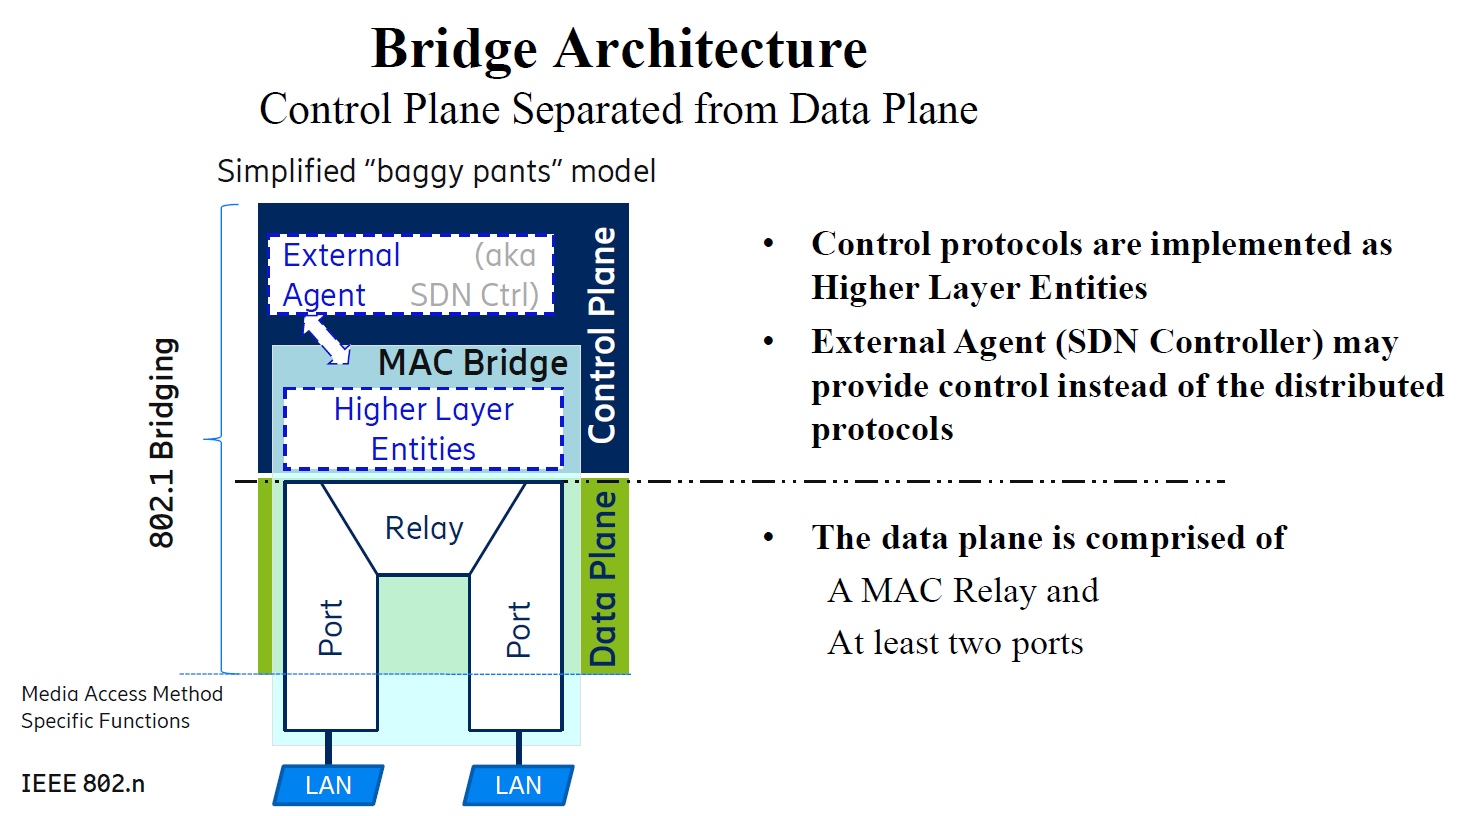
\includegraphics[scale=0.22]{images/Bridge Architecture.png} 
\caption{Bridge Architecture}
\label{fig:Bridge_Architecture}
 \end{figure}
 
 
 \begin{figure}
 
\centering
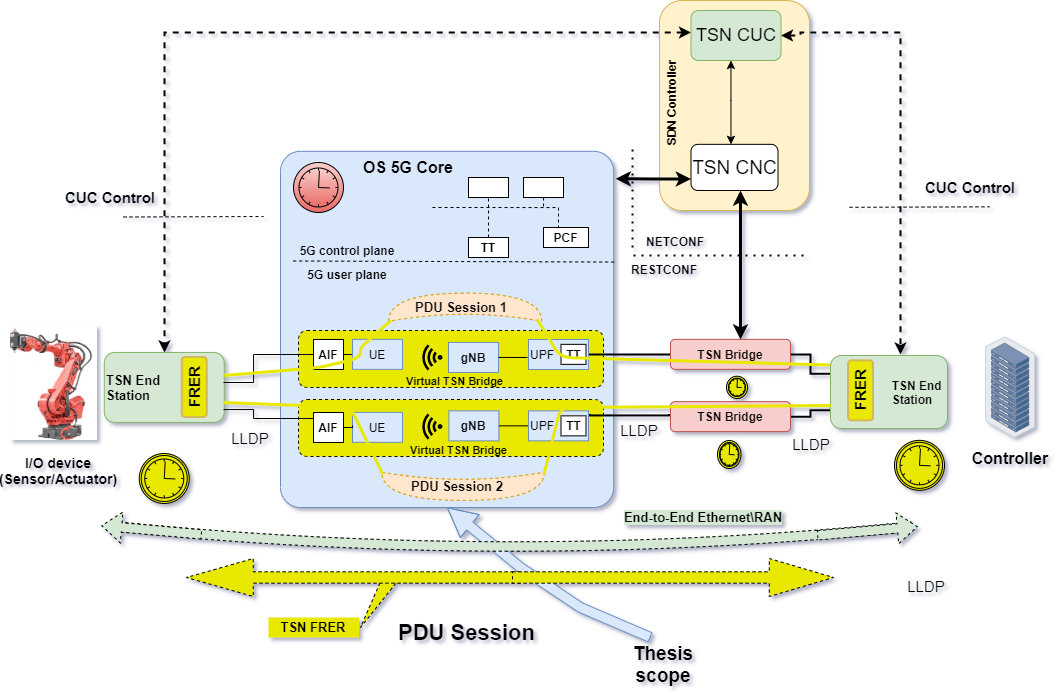
\includegraphics[scale=0.30]{images/OS-5GC-Main.png}
\caption{Open source 5G Core Testbed\cite{Ericsson2019}}
\label{fig:OS-5GC-Main}
  \end{figure}

 
 
 
 
We conclude from the above that The 5GC supports a Protocol Data Unit (PDU) Connectivity Service, i.e., a service that provides the exchange of PDUs between a UE and a data network identified by a Data Network Name (DNN) \cite{ROMMER2020111}. The PDU Connectivity Service is supported via PDU Sessions that are established upon request from the User Equipment (UE), between ingress TSN Translator (TT) and egress TT over Ethernet(not necessarily RAN between 5G base station GNodeB (gNB)  and User Equipment (UE)) as illustrated by figure \textbf{\ref{fig:OS-5GC-Main}}.
Typically, These PDUs can be IP, Ethernet, and Unstructured, besides DNN (Data Network Name) is employed to distinguish various destination networks outside these 5G networks. Figure \textbf{\ref{fig:Simplified_PDU_Session_Establishment_procedure}} represents a simplified PDU Session Establishment call flow, highlighting the key Network Functions included as well as the steps taken in the process \cite{ROMMER2020111}.

 
\begin{figure}
\centering
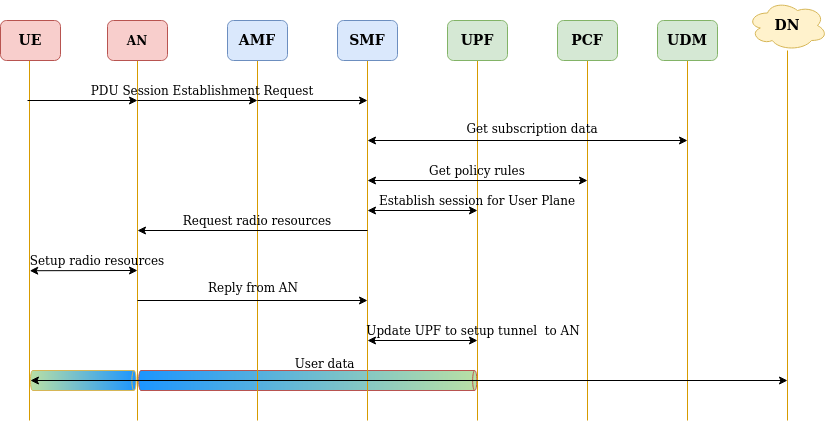
\includegraphics[scale=0.40]{images/Simplified_PDU_Session_Establishment_procedure.png} 
\caption{Simplified PDU Session Establishment procedure \cite{ROMMER2020111}}
\label{fig:Simplified_PDU_Session_Establishment_procedure}
 \end{figure}



 However, all universities and research institutes are closed due to the corona pandemic crisis these days. Nevertheless, Evolved Node B (eNB) or Next Generation NodeB (gNB) provision is impossible because of technical issues and others, related to security and license. Hence, Own approach will be limited to Implementations and Design and Evaluation of a 5G Testbed via Simulation method. Likewise, 5G Service Based Architecture  (SBA) core network will be deployed using docker and docker-compose. Nevertheless, dsTest as a gNB emulator. DsTest offers server emulation and client simulation capabilities for comprehensive testing of 3GPP core network interface functionality and performance\cite{dstest2021}.
 
 

 
 
Two 3GPP 5G research platforms, OpenAirInterface (OAI)  \cite{openairinterface2014}, and Free5GC \cite{Free5gc2019}, are involved in utilizing to deploy 5G Core Network components in virtual and physical machines to achieve Thesis goals.


%\subsection{identification of requirements for TSN over 5G testbeds + comparative analysis of Open Source 5G Core implementations (NextEPC, Free5GC, …)automatic setup of selected open source 5G testbed (LXC, ansible, ...)}

\subsection{SA 5GC Testbed Setup}

Through the simulation approach, different physical and virtual machines will be used. I.e.:
\begin{enumerate}
    \item  On the first stage: Virtualbox is utilized to run several virtual machines, Ubuntu 18.04 operating system and Ubuntu 18.04 Server, to apply the simulation of 5GC  elements (AMF, SMF, NRF, and UPF) provided by OpenAirInterface (OAI) community.
    \item On the second stage: Physical Ubuntu 18.04 OS is utilized to apply the simulation of 5GC  elements, as shown in figure
    \textbf{\ref{fig:Stage2_architecture_of_free5GC}}, provided by Free5GC community If the expected results are not satisfactory in part 1.
    \end{enumerate}
    
    \begin{figure}
\centering
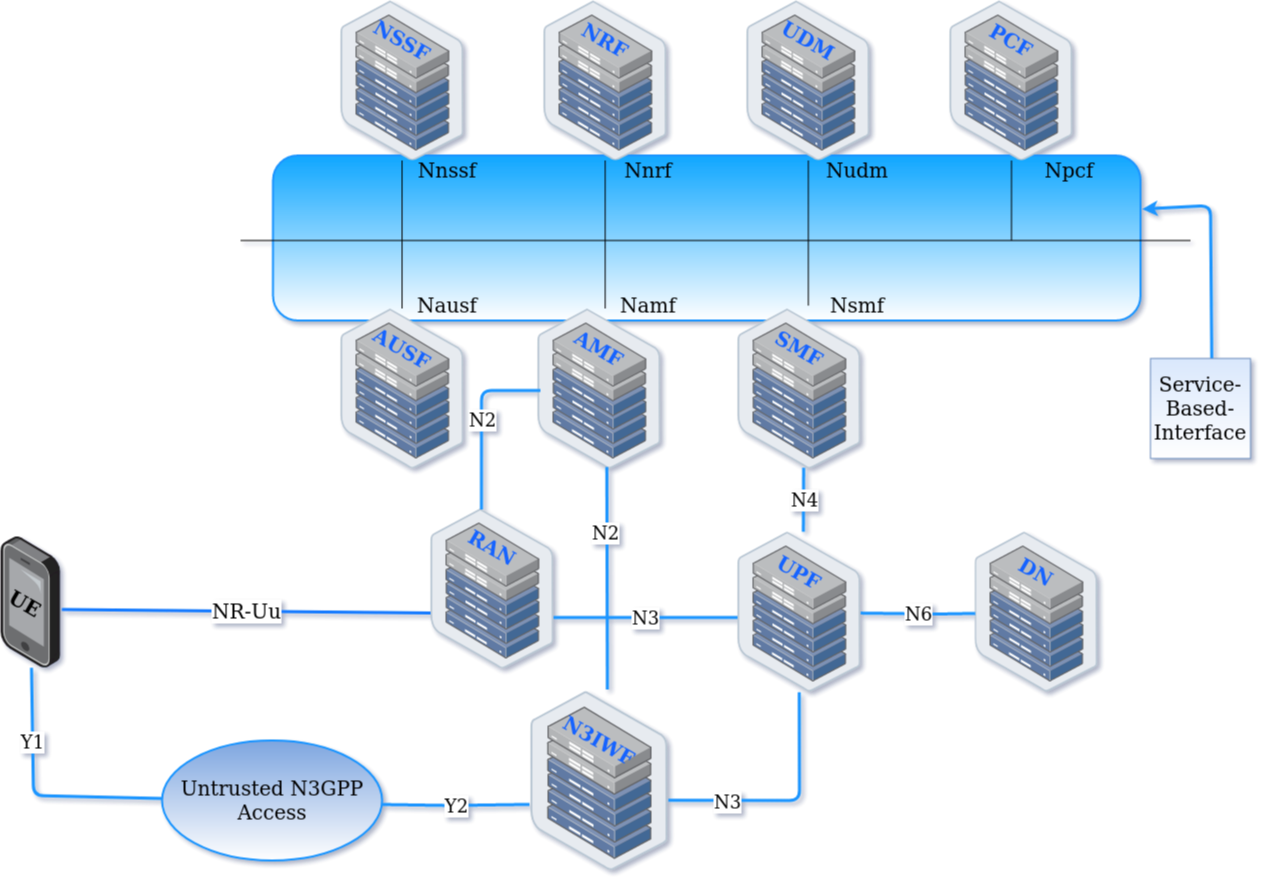
\includegraphics[scale=0.25]{images/Stage2_architecture_of_free5GC.png}
\caption{Stage 2 architecture of free5GC\cite{Free5gc2019}}
\label{fig:Stage2_architecture_of_free5GC}
\end{figure}
    
    
    
\begin{figure}
\centering
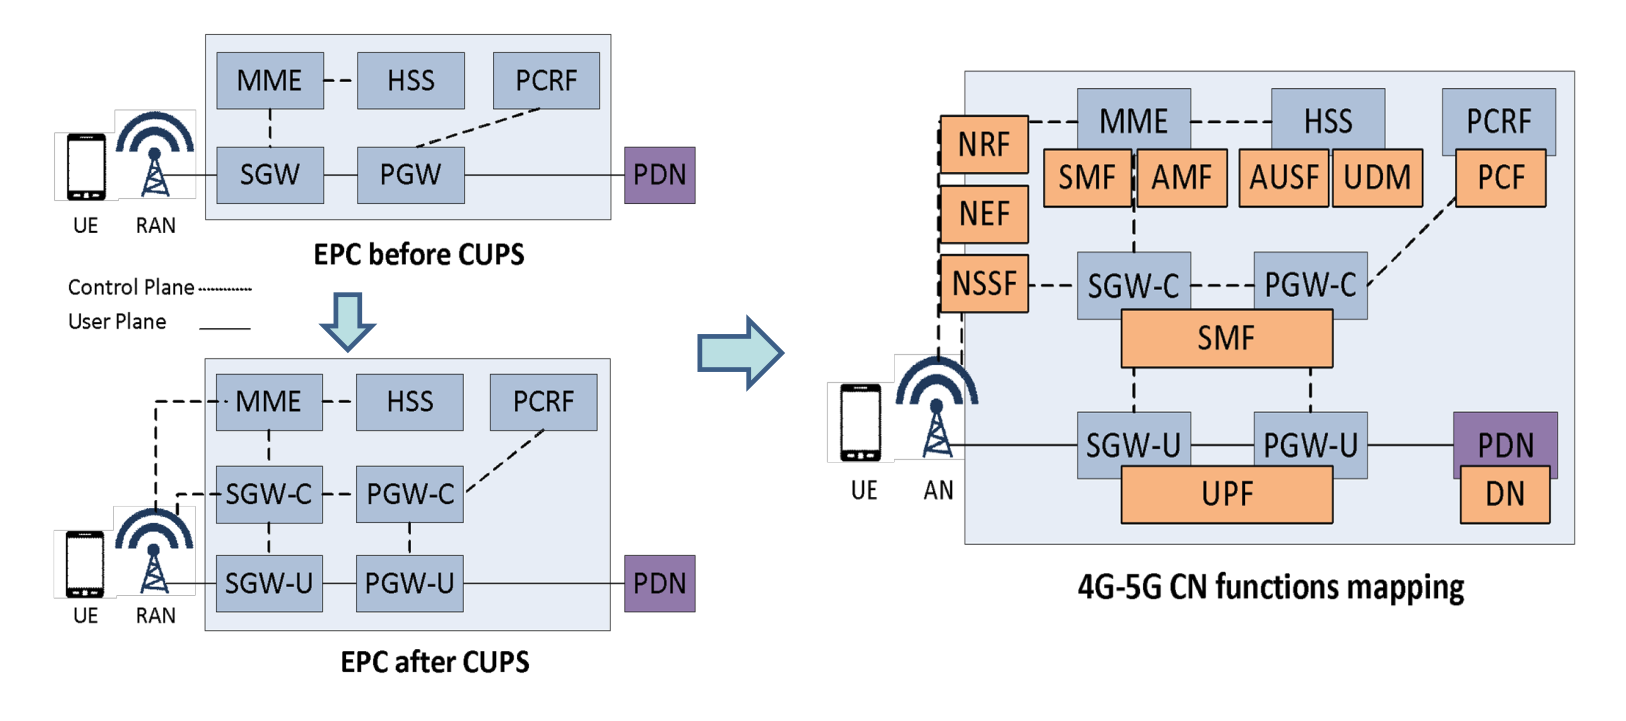
\includegraphics[scale=0.28]{images/oai_epc_core5G1.png}
\caption{5GC Elements corresponding to the 4G \cite{openairinterface2014}}
\label{fig:oai_epc_core5G1}
\end{figure}

    
    
    
    
    
Furthermore, several open source technologies are involved in the study to achieve the aim of this chapter as follows: Docker container, Ansible, Wireshark, Iperf, and dsTest. These terms will be explained in this section and the following sections.


Ansible will make DevOps tasks in this part of the Thesis more effective and less time-consuming. It is an open-source IT automation efficacious tool, which is widely adopted and trusted: because of using simple YAML language and supports different types of infrastructure, e.g., Clouds, Virtual machines. These advantages make it easy for everyone to accept. Furthermore, employ it in all kinds of IT tasks such as configuration management and application deployment. Nevertheless 
, Ansible is agentless or remotely employed.
Besides Ansible components are:
\begin{enumerate}
    \item Ansible Modules: small programs that get executed on target machines.
    \item Ansible Playbook: instructions of the executed programs.
    \item Ansible Inventor: list of hosts where those programs get executed.
\end{enumerate}
Openairinterface (OAI):
The OAI Public License V1.1. Openairinterface permits the researchers, students, and developers to practice and use the OAI 3GPP 5G Core network projects for studying purposes. Figure
\textbf{\ref{fig:oai_epc_core5G1}} depicts the 5GC elements in orange. In other words, it shows fulfilling OAI 5G Core Network components, AMF, SMF, NRF, and UPF (SPGW-U-tiny). Nevertheless, the scenario includes deploying a 5G Service Based Architecture (SBA) core network using docker-compose, dsTest as gNB emulator, attaching and detaching UE, and single public data network (PDN) session establishment.


\begin{figure}
\centering
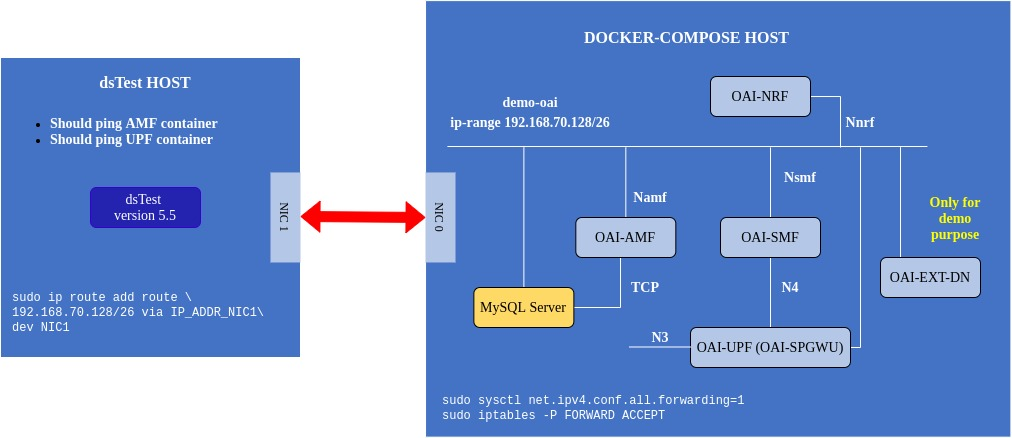
\includegraphics[scale=0.32]{images/OAI5GC_Deployment_using_Docker-Compose_and_Testing_with_dsTest.png}
\caption{5G Core Network Deployment using Docker-Compose and Testing with dsTest \cite{openairinterface2014}}
\label{fig:5GC_Deployment_using_Docker-Compose_and_Testing_with_dsTest}
\end{figure}


The testbed obtains two host machines; As can be noticed in figure
\textbf{\ref{fig:5GC_Deployment_using_Docker-Compose_and_Testing_with_dsTest}}. DsTest host and Docker-compose host, which will be the center of consideration. All 5G core components are running in the Docker-compose host, and they are attached to the same demo-oai. The dstest is deployed in the other machine. The figure shows that the docker-compose host includes an extra container oai-ext-dn, which is only required for the demo goal. Notwithstanding, this container is used in the demo to simulate the downlink traffic. However, because of reasons related to financing, we cannot use a commercial paid gNB emulator (dsTest). Figure \textbf{\ref{fig:5gCN_gnbsim}} shows how can we appropriate gNBsim instead of dstest. Gnbsim is an open-source 5G SA gNB emulator (Rel. 16) for testing 5GS which is written in golang. It simulates NG Application Protocol (NGAP), Non-Access-Stratum (NAS) protocol, and GPRS Tunnelling Protocol User Plane (GTP-U). However, the available gNBsim supports a simulation for one UE and one gNB.




\begin{figure}
\centering
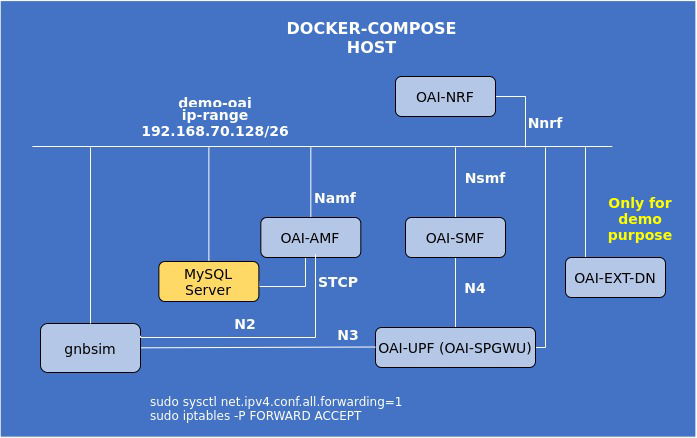
\includegraphics[scale=0.40]{images/5gCN_gnbsim.png}
\caption{5GCN gNBsim  \cite{openairinterface2014}.}
\label{fig:5gCN_gnbsim}
\end{figure}

\clearpage


Pre-requisites of deploying the SA 5GC testbed are described in figure \textbf{\ref{fig:Pre-requisites-oai-cn5g-fed}}. Moreover, the following are the required steps during the setup, which will be explained in detail in the Thesis paper:
\begin{enumerate}
    \item Installation of host operating system Ubuntu 18.04.4 LTS and container operating system Ubuntu 18.04.
    \item Docker engine,  docker-compose, python, and building container images.
    \item Configuring host machines, and configuring OAI 5G Core network functions.
    \item   Deploying OAI 5GC network, getting a gnbsim docker image, and executing gnbsim Scenario.
    \item  Wireshark, and Iperf.
\end{enumerate}
 




\begin{figure}
\centering
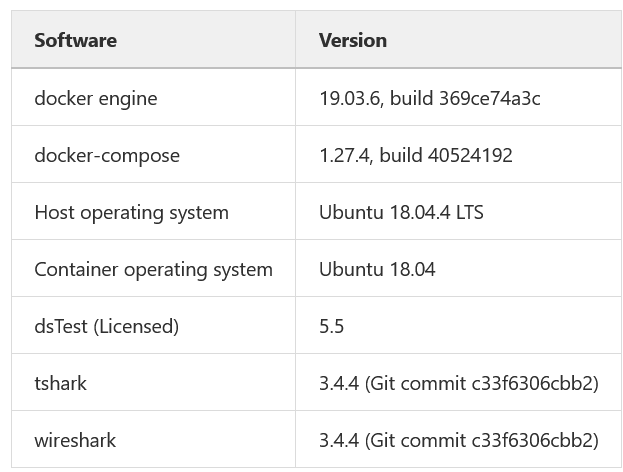
\includegraphics[scale=0.40]{images/Pre-requisites-oai-cn5g-fed.png}
\caption{Pre-requisites OAI 5GCN  \cite{openairinterface2014}.}
\label{fig:Pre-requisites-oai-cn5g-fed}
\end{figure}



 
     
     
   %New colors defined below
\definecolor{codegreen}{rgb}{0,0.6,0}
\definecolor{codegray}{rgb}{0.5,0.5,0.5}
\definecolor{codepurple}{rgb}{0.58,0,0.82}
\definecolor{backcolour}{rgb}{0.95,0.95,0.92}

%Code listing style named "mystyle"
\lstdefinestyle{mystyle}{
  backgroundcolor=\color{backcolour},   commentstyle=\color{codegreen},
  keywordstyle=\color{magenta},
  numberstyle=\tiny\color{codegray},
  stringstyle=\color{codepurple},
  basicstyle=\ttfamily\footnotesize,
  breakatwhitespace=false,         
  breaklines=true,                 
  captionpos=b,                    
  keepspaces=true,                 
  numbers=left,                    
  numbersep=5pt,                  
  showspaces=false,                
  showstringspaces=false,
  showtabs=false,                  
  tabsize=2
}

%"mystyle" code listing set
\lstset{style=mystyle}
  
  
  According to the above, utilizing deployment Docker via Ansible will be more beneficial and operative. Furthermore, the recommendation of Dr.-Ing. Kreuch to present the initially draft instructions of the Ansible playbook of 5GC Network Deployment and Testing with gnbsim will be provided in this section. They are not entirely available yet; because the study and the investigation are ongoing. Nevertheless, this instructions will provide at the abbreviation section in the final thesis paper.  
     
     
     
  Ansible playbook instructions will directly imported and viewed from the files:
  docker-compose.yaml and docker-compose-gnbsim.yaml successively  \cite{openairinterface2014}.
\clearpage


docker-compose.yaml \cite{openairinterface2014}:
%Importing code from file
\lstinputlisting[language=Java, 
caption=docker-compose.yaml\cite{openairinterface2014}.
]{AnsibleFiles/docker-compose.yaml}

\clearpage
Following will be the contents of docker-compose-gnbsim.yaml \cite{openairinterface2014}:

%Importing code from file
\lstinputlisting[language=Java, 
caption=docker-compose-gnbsim.yaml\cite{openairinterface2014}.
]{AnsibleFiles/docker-compose-gnbsim.yaml}

As introduced previously in the draft copy of docker-compose.yaml and docker-compose-gnbsim.yaml both ansible files are preconfigured for executing the gnbsim scenario and will be modified for a test. Then we run the following command to create and launch gnbsim. 
 


%Importing code from file
\lstinputlisting[language=Java, 
caption=Run gnbsim\cite{openairinterface2014}.
]{AnsibleFiles/run_gnbsim.yaml}

Before going to the next step, we need to check that all services' statuses are working fine, as displayed in figure \textbf{\ref{fig:gnbsim_is_healthy}}. 


\begin{figure}
\centering
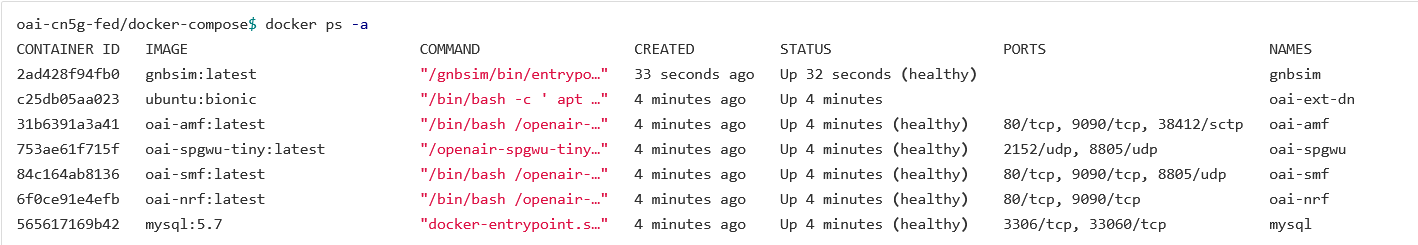
\includegraphics[scale=0.24]{images/gnbsim_is_healthy.png}
\caption{Gnbsim is healthy\cite{openairinterface2014}.}
\label{fig:gnbsim_is_healthy}
\end{figure}
     
     
Momentarily we can implement some traffic tests:
\begin{itemize}
    \item Ping test: Figure \ref{fig:ping_UE_from_external_DN_container} shows us how we ping the UE From the external DN container.
      \item  Iperf test (server/client): 
Between gnbsim UE and the external DN container, we can apply iperf traffic tests because we are able to create any node as an iperf server/client. Figure \ref{fig:iperf_server_traffic_test_between_gnbsim_UE_and_external_DN_node}, figure \ref{fig:iperf_client_traffic_test_between_gnbsim_UE_and_external_DN_node} show the iperf traffic tests and results in the server and client state.
\end{itemize}
   
\begin{figure}
\centering
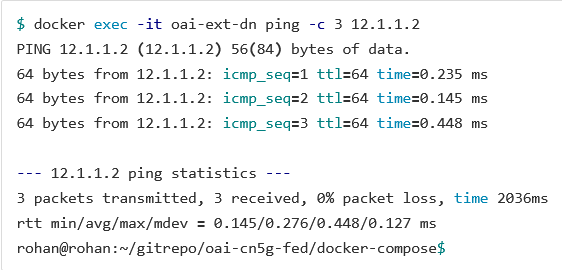
\includegraphics[scale=0.50]{images/ping_UE_from_external_DN_container.png}
\caption{ping UE from external DN container \cite{openairinterface2014}.}
\label{fig:ping_UE_from_external_DN_container}
\end{figure}
 
\begin{figure}
\centering
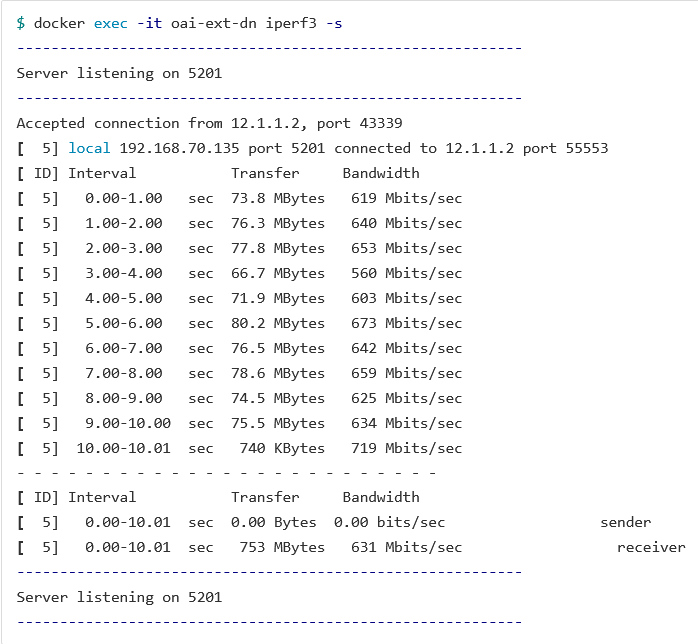
\includegraphics[scale=0.50]{images/iperf_server_traffic_test_between_gnbsim_UE_and_external_DN_node.png}
\caption{Iperf client traffic test between gnbsim UE and external DN node \cite{openairinterface2014}.}
\label{fig:iperf_server_traffic_test_between_gnbsim_UE_and_external_DN_node}
\end{figure}

\begin{figure}
\centering
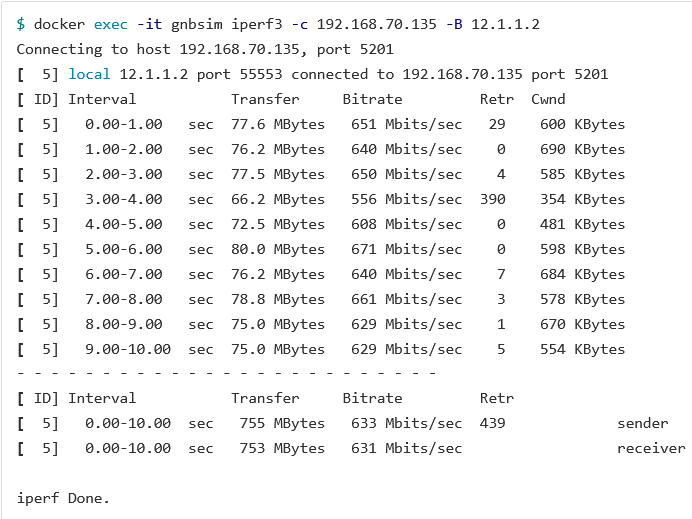
\includegraphics[scale=0.50]{images/iperf_client_traffic_test_between_gnbsim_UE_and_external_DN_node.png}
\caption{Iperf client traffic test between gnbsim UE and external DN node \cite{openairinterface2014}.}
\label{fig:iperf_client_traffic_test_between_gnbsim_UE_and_external_DN_node}
\end{figure}
